\section{Allgemeine Änderungen}

\subsection{Organisatorisches}
\subsubsection{Strutktur der Repositories}
Das ursprüngliche Projekt bestand aus zwei Teilen: der Android App, als lokaler Client, und einem Backend, dessen Service den Bot beinhaltet. Diese Teile waren bisher zusammen in einem einzigen Repository. Das Zusammenlegen hatte eine gewisse Unübersichtlichkeit zur Folge. Daher haben wir für jedes Teilprojekt ein eigenes Repository angelegt. Die Aufteilung zwischen App und Backend wurde beibehalten, lediglich kam noch ein zusätzlicher Teil hinzu, die Service-API-Library. Damit ist die aktuelle Aufteilung auf Github wie folgt:
\begin{itemize}\itemsep0pt
	\item Altes Repository unserer Vorgänger - https://github.com/TeamChatbot/chatbot
	\item Aktuelle Android App - https://github.com/TeamChatbot/Hablame-Android-App
	\item Aktuelle Service-API-Library - https://github.com/TeamChatbot/hablame-service-api
	\item Aktuelles Service-Botbackend - \\https://github.com/TeamChatbot/Hablame-BotBackend
\end{itemize}
Durch diese Aufteilung kann besser und unabhängiger an den einzelnen Teilprojekten gearbeitet werden.

\subsubsection{Aktuelle Aufgabenverteilung auf die Teilprojekte}
Durch das Hinzufügen der Service-API-Library ergibt sich nachfolgend dargestellter Gesamtaufbau.\\
\begin{figure}[h]
	\centering
	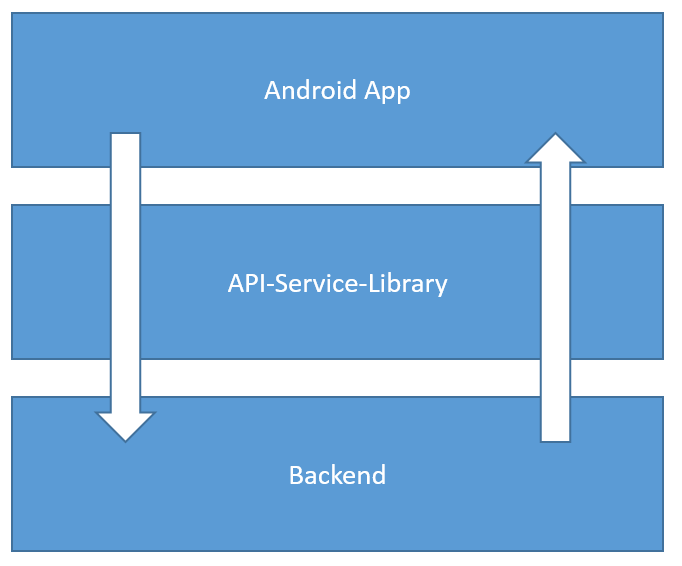
\includegraphics[width=0.7\linewidth]{ks/graphics/arch.png}
	\caption{Gesamtaufbau Hablame}
	\label{fig:arch}
\end{figure}\\
Jedes Teilprojekt behandelt ein Teilproblem des Gesamtsystems.\\
Android App:
\begin{itemize}\itemsep0pt
	\item Umwandlung gesprochener Sprache in Text ("Speech-To-Text")
	\item Umwandlung von Text in gesprochene Sprache ("Text-To-Speech")
	\item Weiterleiten der Informationen mittels der API-Service-Library an das Backend
\end{itemize}
API-Service-Library:
\begin{itemize}
	\item Erstellen der Anfragen an das Backend
	\item Weitergabe der Backend-Antworten an das aufrufende System
\end{itemize}
Backend:
\begin{itemize}
	\item Hosting und Konfiguration des Chatbots
	\item Auswerten der Serviceanfragen
\end{itemize}

\subsection{Dokumentation im Allgemeinen}
Für die Dokumentation gibt es nun mehrere Anlaufstellen. In Redmine gibt es ein integriertes Wiki welches wir bereits mit einigen Informationen zu allgemeine Dingen wie Logindaten und den einzelnen Repositories, aber auch zu genutzten Technologien wie beispielsweise das Git-System gefüllt.\footnote{Projekt Wiki in Redmine: http://194.95.221.229/redmine/projects/hablame/wiki/}
Zusätzlich zu dem Wiki gibt es in jedem Repository ein Readme, das nochmal zusätzlich einen Überblick über das dortige Projekt gibt.\\
Die Dokumentation des Programmcodes ist mittels dem Java Tool JavaDocs umgesetzt worden. Die damit generierten Dokumentationsseiten sind im jeweiligen Repository auf Github zu finden.

\subsection{Unit Testing}
Neu ist auch das, bisher nicht beachtete, automatisierte Testen des Programmcodes. Hierfür wird auf das Java Framework JUnit zurückgegriffen.\footnote{Projektseite von JUnit: http://junit.org/} Durch das Nutzen eines solchen Frameworks ist es möglich automatisiert Programmcode auf die korrekte Ausführung zu testen. Gerade in einem großen System wie das Backend nimmt das einiges an arbeit ab, während es die Wartbarkeit deutlich erhöht.\\
Aktuell wird es sowohl im Backend, als auch in der Service-API-Library genutzt.\\
Im Backend werden zusätzlich noch die Mockito Bibliotheken genutzt, da es mit diesen ermöglicht wird zusätzlich noch die Controller-API zu testen, welche den Chatbot von außen über Requests erreichbar und ansprechbar macht.

\subsection{Build Management mit Maven}
Ein Problem im bisherigen Projekt war, dass Abhängigkeiten und der Buildvorgang nicht zentral geregelt wurden. So wurden genutzte Bibliotheken als Jar-Archive eingebunden. Dies hat zur Folge das diese Bibliotheken zu meist händisch in das Arbeitssystem geladen werden müssen. Um dies zu vereinfachen und den Buildvorgang zu vereinheitlichen wird im Backend sowie der Service-API-Library nun das Build Management Tool Maven verwendet.\footnote{Projektseite von Maven: https://maven.apache.org/} Somit gibt es jetzt in beiden Projekten einen einheitlichen Punkt für die Konfiguration der Abhängigkeiten und des Buildvorgangs, die pom.xml.

